
\chapter{Tests}
\label{chap:test}

\section{Unit tests}

During this project I did some unit tests to preserve the code during the development. But, I had a lot of difficulties to tests user interface features, so I chose, on Simon advice, to don't tests them. However, I have tested all other functions used in the plugin.
~\\

To do this unit tests, I used junit and an eclipse feature EclEmma which permit to see the coverage of code during unit tests. On the figure \ref{fig:coverage}, you can see the result of the coverage show by EclEmma about my project.
~\\

First of all, you can see the package json was not well tested. This package was written by stleary\cite{json}, so I didn't write unit tests for this package.

Then, packages org.ensta.uml.sim.views.features and org.ensta.uml.sim.views.design only contain class which do action on the user interface. So I didn't tests them.

After this remarks, it is possible to notice that I tested more then 80\%\footnote{It is the usual value of acceptable coverage} of the code use in other classes.


\begin{figure}[h]
  \centering
  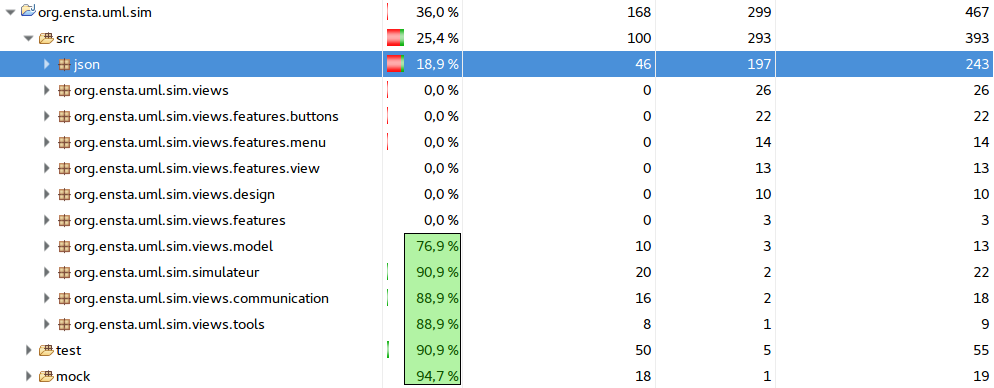
\includegraphics[width=\linewidth]{coverage}
  \caption{Coverage view of my project}
  \label{fig:coverage}
\end{figure}

\section{Integration tests}

I also did some integration tests to verify that I respect one of my constraint, be installable  in all platform (Windows, Linux, Apple).

During all my project I verified that my plugin could be use on my own computer without the eclipse developer environment. I have a Ubuntu 16.04 LTS.

Then, at the end of my project, I tried to use this plugin on other platform. To do that, I use virtual machine with VirtualBox. I tested on a Windows virtual machine with W7 (figure \ref{fig:windows}), and a Kali virtual machine based on Debian (figure \ref{fig:kali}). However, I didn't try on OSX because I didn't find a OSX virtual machine on the internet.

\begin{figure}[h]
  \centering
  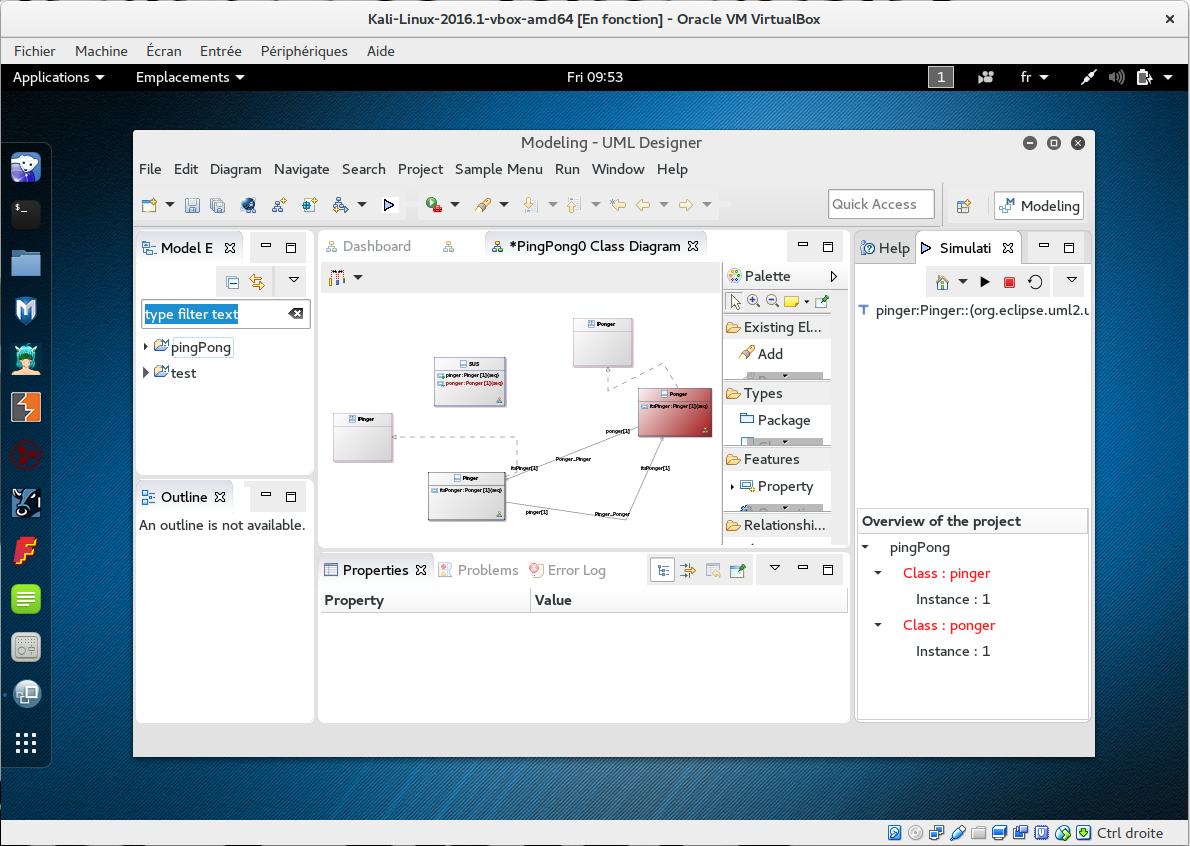
\includegraphics[width=\linewidth]{kali}
  \caption{Screen-shot of the kali virtual machine}
  \label{fig:kali}
\end{figure}

\begin{figure}[h]
  \centering
  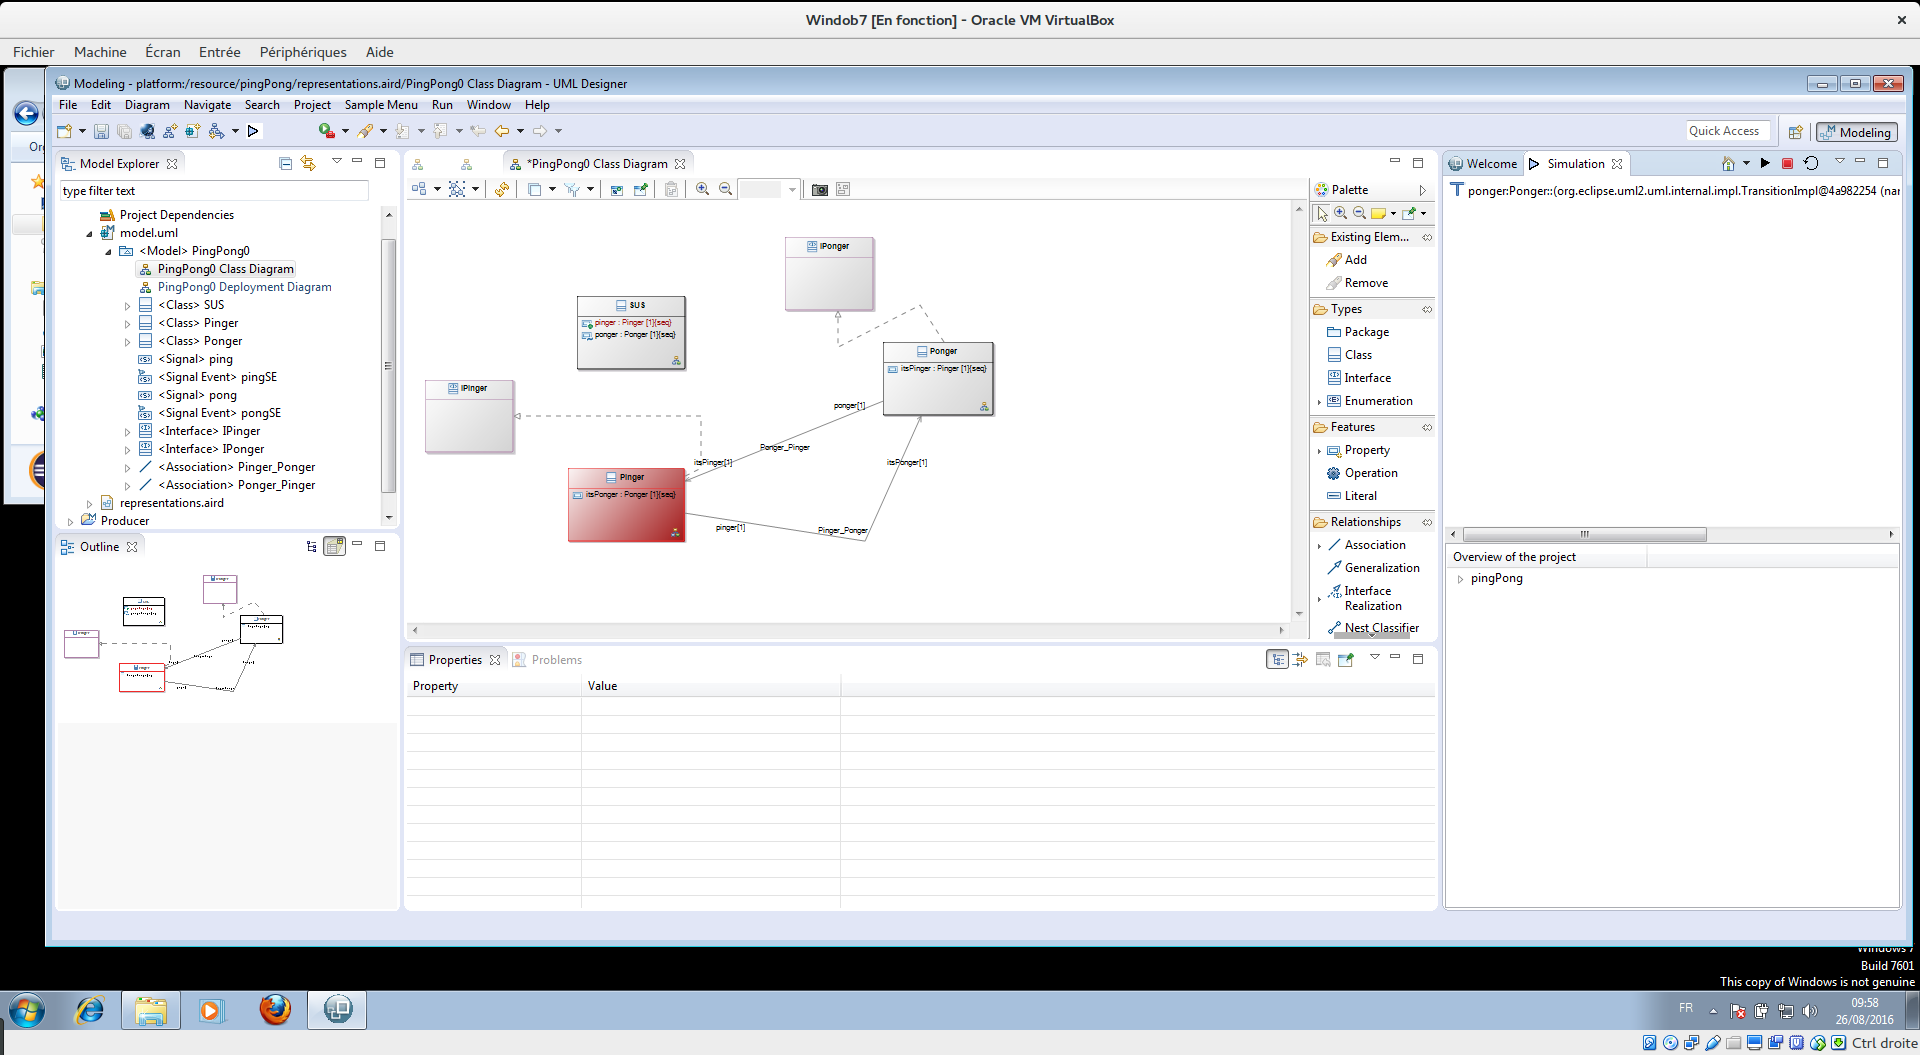
\includegraphics[width=\linewidth]{windows}
  \caption{Screen-shot of the Windows virtual machine}
  \label{fig:windows}
\end{figure}


%%% Local Variables:
%%% mode: latex
%%% TeX-master: "../rapport_de_base"
%%% End:
